\documentclass[final,5p,times,twocolumn,authoryear]{elsarticle}

\usepackage{amssymb}
\usepackage{url}
\usepackage{float}

\begin{document}

\begin{frontmatter}

  \title{WE NEED A TITLE HEERE ???}

\author[first]{André Costa}
\author[second]{Celso Ribeiro}
\author[third]{David Mendes}
\affiliation{organization={ISCTE – Instituto Universitário de Lisboa},
            country={Portugal}}

  \begin{abstract}
    This article aims to summarize the approach and results of \cite{Stacking}, in which the authors explore employing stacking, boosting, and blending machine learning algorithms to predict student performance in large-scale assessments based on a wide range of predictors and compare their performance.
  \end{abstract}

  \begin{keyword}
    PISA \sep Machine learning \sep Stacking \sep Boosting \sep Blending \sep Ensemble
    learning
  \end{keyword}

\end{frontmatter}


% \linenumbers

\section{introduction}\label{sec:introduction}
Lorem ipsum dolor sit amet, consectetur adipiscing elit, sed do eiusmod tempor incididunt ut labore et dolore magna aliqua. Ut enim ad minim veniam, quis nostrud exercitation ullamco laboris nisi ut aliquip ex ea commodo consequat. Duis aute irure dolor in reprehenderit in voluptate velit esse cillum dolore eu fugiat nulla pariatur. Excepteur sint occaecat cupidatat non proident, sunt in culpa qui officia deserunt mollit anim id est laborum.~\cite{markovichz}.





\section{Business Understanding}\label{sec:business_understanding}

Large‑scale international assessments such as the \textbf{Programme for International Student Assessment (PISA)} provide policy‑makers with uniquely comparable evidence on the cognitive skills of 15‑year‑olds.  Yet ministries and school leaders frequently lack timely, granular diagnostics that explain \emph{why} some learners underperform while others excel.  Our project addresses this gap by developing an AI‑based early‑warning model that flags students at risk of \textit{low achievement} in mathematics, science, and reading using the publicly released \textbf{PISA 2022 Student Questionnaire} micro‑data set.

The business—or, more precisely, educational policy—problem can be stated as follows:

\begin{quote}
    \emph{“Given a fixed budget for instructional support, how can education systems proactively target pedagogical and socio‑emotional interventions toward students most likely to obtain low PISA scores, thereby reducing grade repetition and narrowing equity gaps?”}
\end{quote}

Operationalising this question involves three goals:

\begin{enumerate}
    \item \textbf{Predictive analytics}: learn a mapping from student‑level contextual variables ($\mathbf{X}$) to performance deciles ($y$) that generalises across participating economies.
    \item \textbf{Actionable insights}: identify the subset of predictors with the \emph{strongest marginal contribution} to low performance, so interventions can be prioritised.
    \item \textbf{Benchmarking}: compare the risk profiles of repeating students against high performers, highlighting differences that may travel across national borders.
\end{enumerate}

\paragraph{Key findings to date.}
Exploratory correlation and feature‑importance screens on $\sim700$ candidate variables reveal four robust signals:

\begin{itemize}
    \item \textbf{Socio‑economic status (ESCS)} represents the largest single share of variance in low scores; a one‑decile drop in ESCS increases the probability of bottom-quartile performance by 6 to 8 pp.
    \item \textbf{Sense of school belonging} and \textbf{test‑skill confidence} together exert a comparable influence, especially on mathematics.
    \item \textbf{Late school entry} (age $>$ 7) and \textbf{grade repetition history} exhibit strong conditional correlations with poor science outcomes.
    \item Contrary to conventional belief, \textbf{time‑spent‑on‑homework} shows only a weak negative correlation once SES and self‑efficacy are controlled.
\end{itemize}

These empirical patterns motivate our choice of ensemble models (stacking, gradient boosting) that handle high‑dimensional, collinear, and partially missing data while producing interpretable feature importances.

\paragraph{Why cross‑country comparison matters.}
Although PISA is standardised, the institutional context in which 15‑year‑olds learn varies considerably:

\begin{description}
    \item[England] operates a \emph{comprehensive system} with Key Stages and externally set GCSE exams at age 16; grade repetition is rare and pupils can select specialised pathways post‑16.\footnote{\url{https://b28mathstutor.co.uk/how-the-english-school-system-works/}}
    \item[Singapore] employs a differentiated but tightly sequenced route from Primary 1 through O‑Level/Integrated Programme, emphasising streaming and national examinations.\footnote{\url{https://en.wikipedia.org/wiki/Education_in_Singapore}}
    \item[Germany] divides students after Grade 4 into multiple secondary pathways (Gymnasium, Realschule, Hauptschule); grade repetition is relatively common and tracked.\footnote{\url{https://www.studying-in-germany.org/german-education-system/}}
    \item[United States] offers a largely \emph{comprehensive K–12} model governed by state standards and the Carnegie unit; social promotion policies reduce formal repetition but conceal skill deficits.\footnote{\url{https://en.wikipedia.org/wiki/Education_in_the_United_States}}
\end{description}


Recognising such systemic contrasts is essential: a “risk factor” identified in one jurisdiction (e.g.\ after‑school tutoring hours in Shanghai) may not be policy‑controllable in another (e.g.\ England, where after‑school tuition is privately financed).  Therefore, our modelling pipeline includes country‑specific fixed effects and studies interaction terms between student attributes and system‑level dummies.

\paragraph{What teaching strategies enhance reading performance?}
Insights from \textbf{PISA 2018} contextual data offer valuable evidence. According to the teacher questionnaire, strategies such as \emph{explicit reading instruction}, \emph{activating prior knowledge}, and \emph{engaging students in metacognitive practices} were correlated with higher reading performance. From the student perspective, respondents who reported frequent use of \emph{discussions about texts}, \emph{clarity in lesson structure}, and \emph{constructive feedback} also scored higher on average. Interestingly, while both teachers and students pointed to structured and cognitively activating instruction as beneficial, teachers tended to emphasize planning and scaffolding, whereas students highlighted motivation and classroom climate. This discrepancy reinforces the importance of triangulating perspectives in education data analytics.

\paragraph{Profiling students in vocational education tracks.}
Another avenue of investigation focuses on students enrolled in \textbf{vocational and professional training programs} as defined in PISA. Historically, these students perform lower in mathematics than those in general education tracks. Variables explaining this gap include reduced parental education, lower socio-economic status, and limited exposure to advanced mathematics content. However, over successive cycles of PISA (2012–2018), some countries have seen marginal gains for vocational-track students—particularly where applied mathematics and contextualised problem-solving were integrated into the curriculum. Our model incorporates program type as a categorical feature and enables interaction testing with SES, gender, and country-level effects to better understand these evolving patterns.


\paragraph{Success criteria.}
From a business‑value perspective, we deem the CRISP‑DM \emph{Business Understanding} phase complete when we can:

\begin{itemize}
    \item articulate the decision points (resource targeting, curriculum design) that model outputs will inform;
    \item translate model metrics into cost–benefit terms for ministries (e.g.\ reduction in misallocated tutoring hours per \$100k invested in data collection);
    \item outline ethical safeguards to prevent algorithmic bias against vulnerable groups.
\end{itemize}

Establishing this shared understanding with stakeholders ensures that the subsequent CRISP‑DM phases—Data Understanding, Data Preparation, Modelling, and Evaluation—remain anchored to actionable educational impact.


Building on this policy motivation, the empirical backbone of our work is the study by \cite{Stacking}, which exploits the same \textbf{PISA 2022 Student Questionnaire} micro‑data.  Their benchmark investigation compares three ensemble‑learning families—\emph{stacking}, \emph{boosting}, and \emph{blending}—for predicting mathematics, reading, and science scores.  Stacking aggregates the outputs of diverse base learners into a meta‑model, boosting trains learners sequentially so each iteration corrects the residuals of the previous one, while blending fits base models on a hold‑out validation set before meta‑aggregation.  \citeauthor{Stacking} report that stacking consistently yields the lowest error metrics (MAPE, MAE, MSE), a finding that motivates our own choice of stacked architectures for early‑warning classification.


\section{Related Work}\label{sec:related_work}

Lorem ipsum dolor sit amet, consectetur adipiscing elit, sed do eiusmod tempor incididunt ut labore et dolore magna aliqua. Ut enim ad minim veniam, quis nostrud exercitation ullamco laboris nisi ut aliquip ex ea commodo consequat. Duis aute irure dolor in reprehenderit in voluptate velit esse cillum dolore eu fugiat nulla pariatur. Excepteur sint occaecat cupidatat non proident, sunt in culpa qui officia deserunt mollit anim id est laborum. ~\cite{matlabpb}
Lorem ipsum dolor sit amet, consectetur adipiscing elit, sed do eiusmod tempor incididunt ut labore et dolore magna aliqua. Ut enim ad minim veniam, quis nostrud exercitation ullamco laboris nisi ut aliquip ex ea commodo consequat. Duis aute irure dolor in reprehenderit in voluptate velit esse cillum dolore eu fugiat nulla pariatur. Excepteur sint occaecat cupidatat non proident, sunt in culpa qui officia deserunt mollit anim id est laborum. ~\cite{KOLM2014356}
\section{Data Preparation}\label{sec:data_preparation}

After the previous analysis, we proceeded to the data preparation stage, where the dataset was refined for the modelling phase.

\subsection{Question 1}

We began by importing the complete raw dataset and applied the results of our previous analysis to select the most relevant features.

First, we removed unnecessary variables according to the following criteria:
\begin{itemize}
    \itemsep0em
    \item Variables with more than 70\% missing values.
    \item Students from England, due to differences in their education system.
\end{itemize}

\noindent
Next, we introduced the following variables:
\begin{itemize}
    \itemsep0em
    \item \texttt{Avg Math Result}
    \item \texttt{Avg Reading Result}
    \item \texttt{Avg Science Result}
\end{itemize}

\noindent
These were calculated as the average of the respective plausible values (PV1 to PV10) for each student.
We also removed the subscales of Mathematics, as their information is already captured by the aggregated Math Result score.

Then, we grouped the \texttt{Country (CNT)} variable into three categories to reduce high dimensionality:
\begin{itemize}
    \itemsep0em
    \item Above Average
    \item Average
    \item Below Average
\end{itemize}
This grouping was based on the average performance of students in each country across all subjects.

Using this new cleaned dataset, we created a correlation chart to visualize which features have a strong correlation with the target variable \texttt{Avg Math Result}.
In Figure \ref{fig:correlation_chart_repeating} and Figure \ref{fig:correlation_chart_not_repeating}, we can see the correlation obtained for the non-repeating and repeating students, respectively.

\begin{figure}[H]
    \centering
    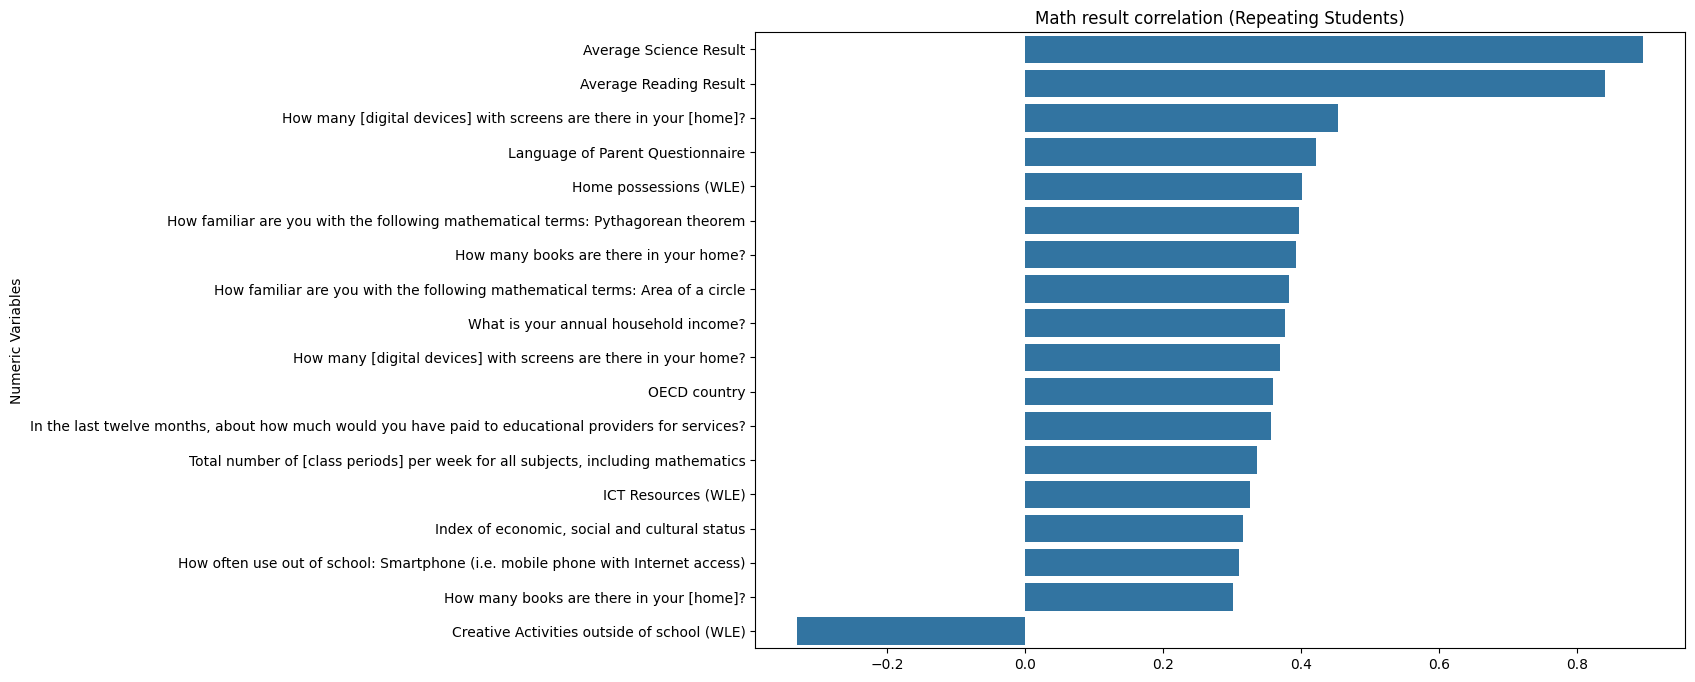
\includegraphics[width=0.48\textwidth]{figures/Q1_repratingcorrelations.png}
    \caption{Correlation matrix showing the relationship between selected features and the target variable \texttt{Avg Math Result} for repeating students.}
    \label{fig:correlation_chart_repeating}
\end{figure}


\begin{figure}[H]
    \centering
    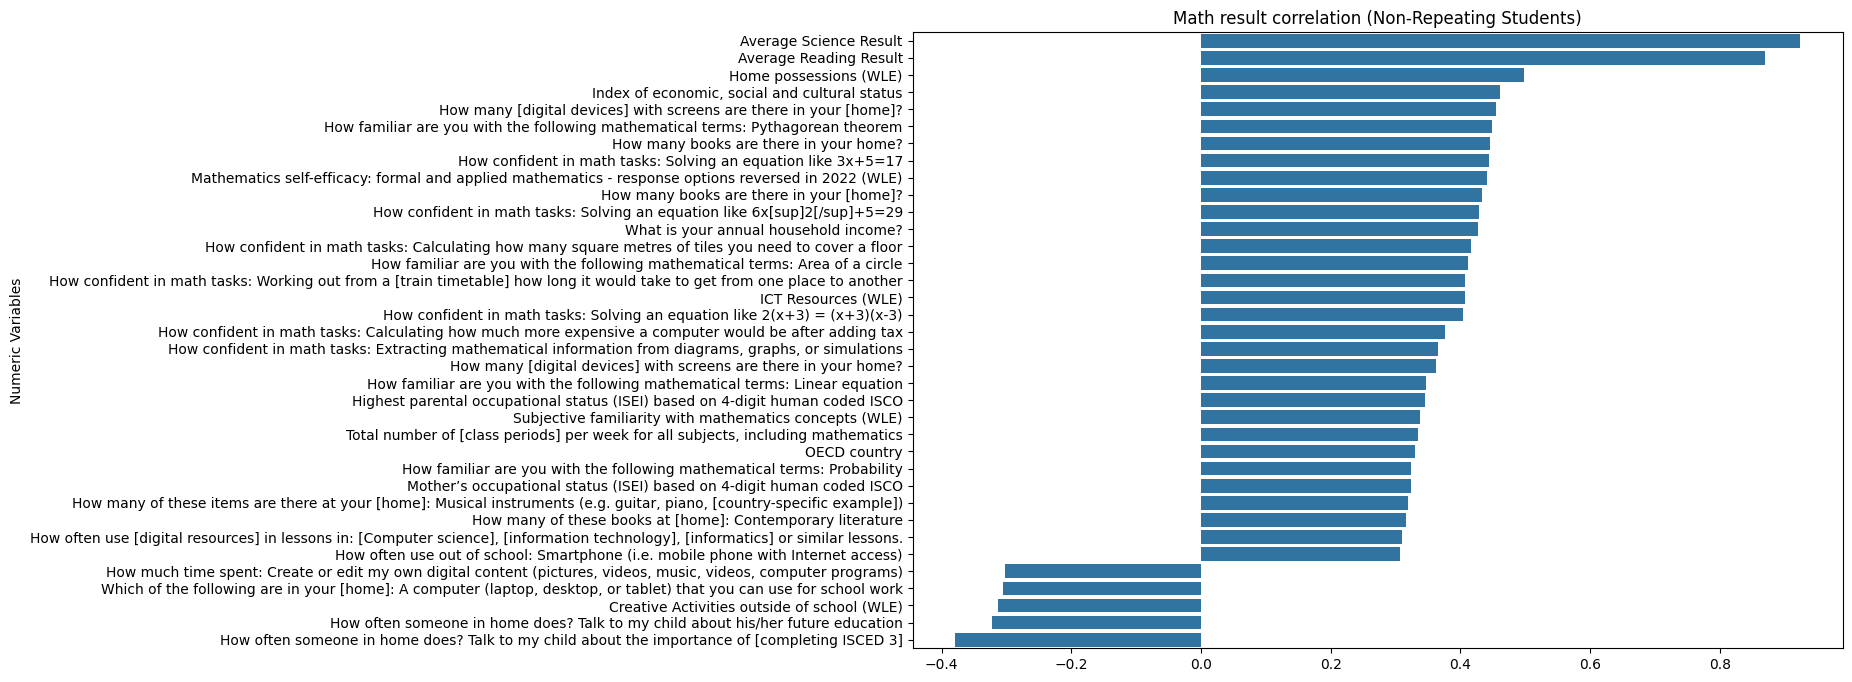
\includegraphics[width=0.48\textwidth]{figures/Q1_nonrepeatingcorrelations.png}
    \caption{Correlation matrix showing the relationship between selected features and the target variable \texttt{Avg Math Result} for non repeating students.}
    \label{fig:correlation_chart_not_repeating}
\end{figure}


Based on this analysis, we selected a mix of features that were significantly correlated with the target variable in either group. Additionally, we included the \texttt{Country (CNT)} variable to account for geographic effects.
The resulting dataset contains 40 variables and 613 744 rows of data, and serves as the foundation for the modelling phase.
\section{Related Work}\label{sec:related_work}

Lorem ipsum dolor sit amet, consectetur adipiscing elit, sed do eiusmod tempor incididunt ut labore et dolore magna aliqua. Ut enim ad minim veniam, quis nostrud exercitation ullamco laboris nisi ut aliquip ex ea commodo consequat. Duis aute irure dolor in reprehenderit in voluptate velit esse cillum dolore eu fugiat nulla pariatur. Excepteur sint occaecat cupidatat non proident, sunt in culpa qui officia deserunt mollit anim id est laborum. ~\cite{matlabpb}
Lorem ipsum dolor sit amet, consectetur adipiscing elit, sed do eiusmod tempor incididunt ut labore et dolore magna aliqua. Ut enim ad minim veniam, quis nostrud exercitation ullamco laboris nisi ut aliquip ex ea commodo consequat. Duis aute irure dolor in reprehenderit in voluptate velit esse cillum dolore eu fugiat nulla pariatur. Excepteur sint occaecat cupidatat non proident, sunt in culpa qui officia deserunt mollit anim id est laborum. ~\cite{KOLM2014356}

\bibliographystyle{elsarticle-harv}
\bibliography{main}

\end{document}

\endinput
